\def\QRCODE{TB_IPR_TUT.IMG.stereology_matlabqrcode.png}
\def\QRPAGE{http://www.iptutorials.science/tree/master/TB_IPR/TUT.IMG.stereology/matlab}
\mcorrectionsection{Matlab correction}

\subsection{Classical measurements of stereology }

\subsubsection{Population of disks}
To generate a given number of overlapping disks, the following procedure can be used. Result is shown in Fig. \ref{fig:stereology:matlab:disk2}.

\begin{matlab}
% generates population of disks
function I = popDisks(nb_disks, S, Rmax)
% nb_disks: number of disks
% S: size of the spatial support
% Rmax: maximum radius of disks
% I: result, binary image of size SxS

I = zeros(S);

positions = randi(S, nb_disks, 2);
radii     = rand(nb_disks, 1) * Rmax;

[X, Y] = meshgrid(1:S, 1:S);
for i=1:nb_disks
    
    I2 = ((X-positions(i,1)).^2 + (Y-positions(i,2)).^2) <= radii(i).^2;
    I = I | I2;
end
\end{matlab}

\begin{figure}[htbp]
 \centering
 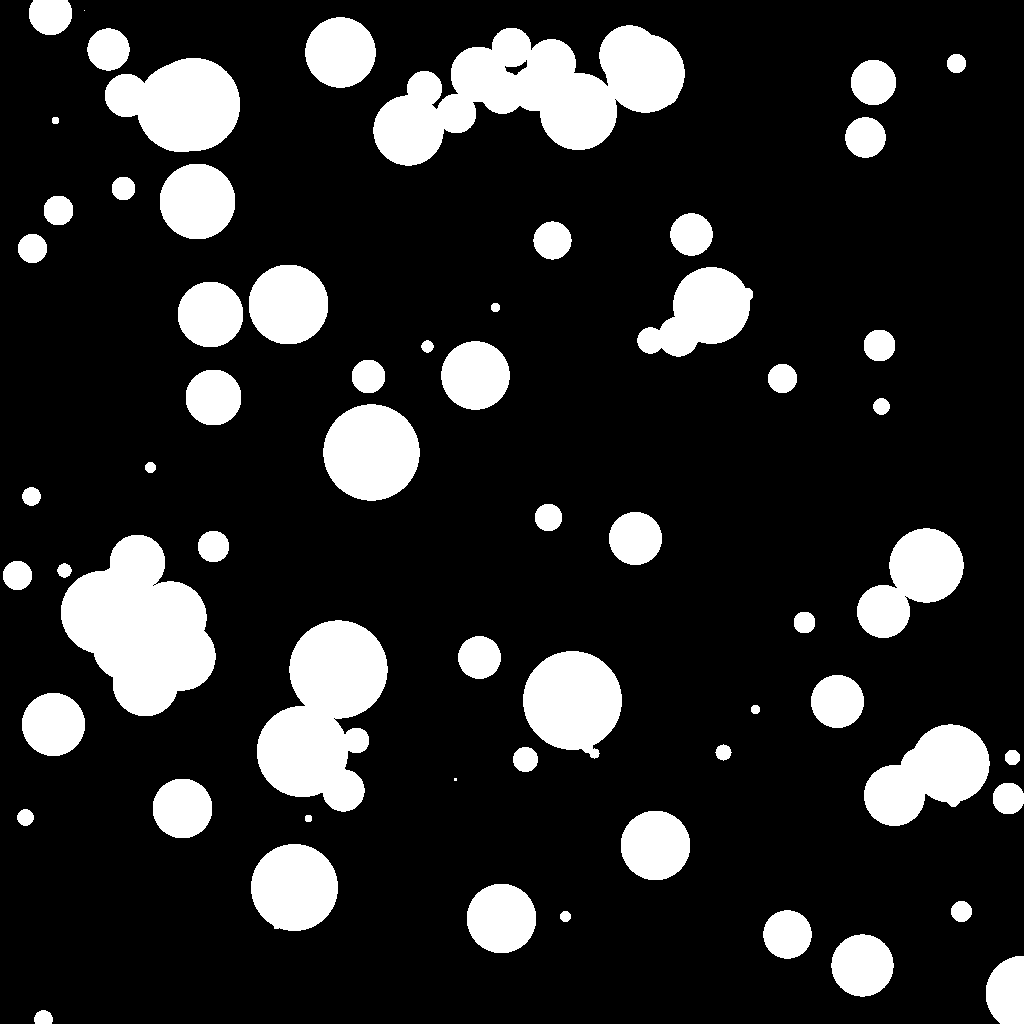
\includegraphics[width=5cm]{disks2.png}
 \caption{Random population of disks in a rectangle.}
 \label{fig:stereology:matlab:disk2}
\end{figure}


\subsubsection{Area fraction}
The 2-D binary image containing the population of disks is loaded or generated by the previous method:
\begin{matlab}
A=double(imread('disks.bmp')/255);
\end{matlab}

Then the points are randomly chosen and the measures are taken
\begin{matlab}
% Points where the measures are performed
nbPoints=1000;
P = randi(size(A,1), nbPoints, 2);

% Do the measures
probes=0;
for i=1:nbPoints
    if A(P(i,1), P(i,2)) == 1
        probes = probes + 1;
    end
end

% the area of the objects can be measured by the ratio of probes/nbPoints
PP = probes/nbPoints;
disp(['PP: ' num2str(c)])
\end{matlab}

This value has to be compared to the real number of pixels:

\begin{matlab}
AA = bwarea(A)/(size(A,1) * size(A,2));
disp(['AA: ' num2str(r)])
\end{matlab}


\begin{mwindow}
>>PP: 0.369
>>AA: 0.36576
\end{mwindow}


\subsubsection{Length per area}
This evaluation highly depends on the result of the perimeter evaluation that depends on the connectivity chosen. The Fig.\ref{fig:stereology:matlab:probeline} illustrates the different steps for evaluating $P_L$.
\begin{matlab}
% create an image with lines
probe=zeros(512,512);
probe(20:50:end-20,20:end-20)=1;
lines=probe.*A;

% detect number of segments
points=abs(conv2(lines,[1 -1 0], 'same'));

disp(['pi*PL/2 : ' num2str(sum(points(:))/sum(lines(:))*pi/2)])
disp(['LA: ' num2str(sum(sum(bwperim(A)))/bwarea(A))])
\end{matlab}

\begin{figure}[htbp]
 \centering
 \subfloat[Probe lines.]{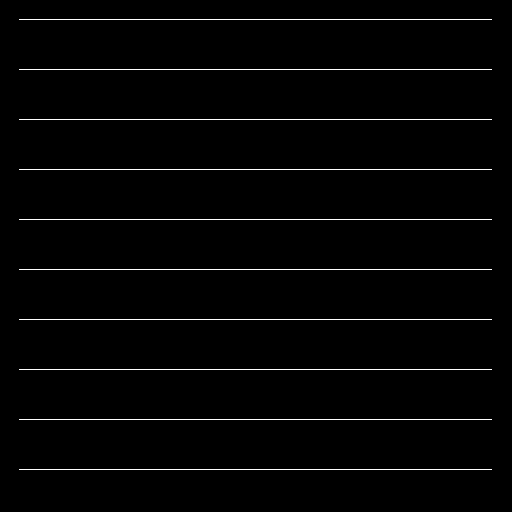
\includegraphics[width=.3\linewidth]{probe_line.png}}\hfill
 \subfloat[Intersection with binary set.]{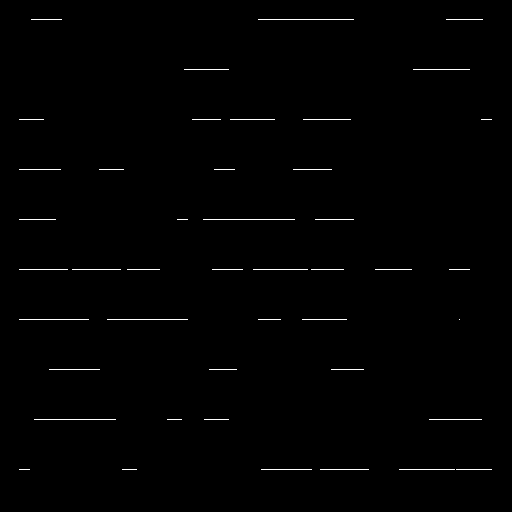
\includegraphics[width=.3\linewidth]{probe_line_2.png}}\hfill
 \subfloat[Location of intersection with the surface of the binary set.]{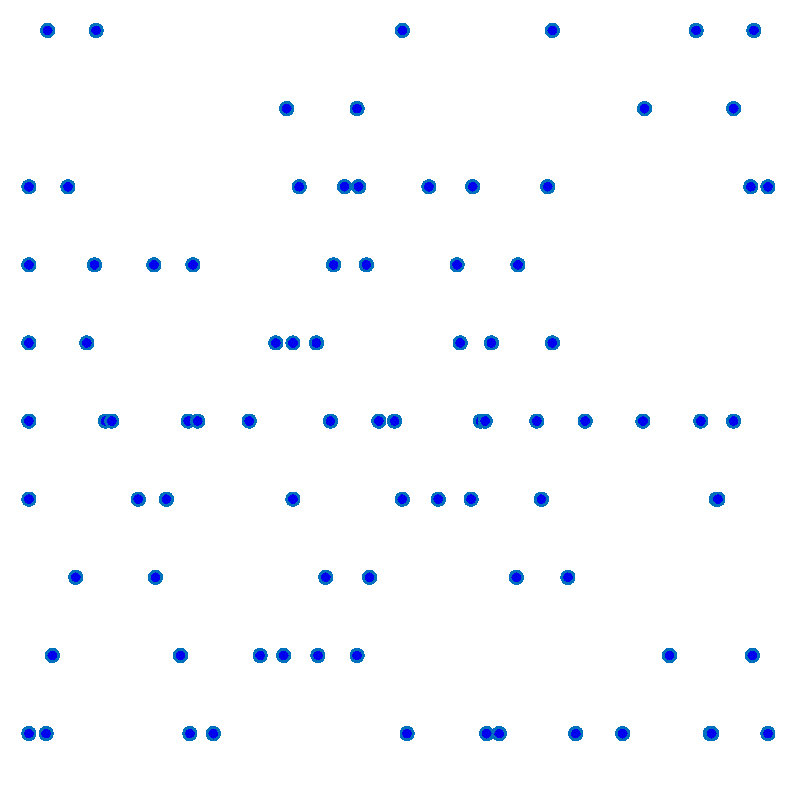
\includegraphics[width=.3\linewidth]{probe_line_3.pdf}}
 
 \caption{Probe lines.}
 \label{fig:stereology:matlab:probeline}
\end{figure}

% results
\begin{mwindow}
>>pi*PL/2 : 0.078406
>>LA: 0.067719
\end{mwindow}


\subsubsection{Volume fraction}
This measure is more precise and is the equivalent of the area fraction.
\begin{matlab}
spheres = load('spheres.mat');
VV = sum(spheres.A(:)) / (size(spheres.A,1) * size(spheres.A,2) * size(spheres.A,3));
probe = zeros(size(spheres.A));
probe(10:50:end-10, 10:end, 10:end) = 1;

s = sum(probe(:));
probe = probe .* spheres.A;
AA= sum(probe(:)) / s;
disp(['VV=' num2str(VV)])
disp(['AA=' num2str(AA)])
\end{matlab}

\begin{mwindow}
>>VV=0.050185
>>AA=0.052769
\end{mwindow}


\subsection{Random chords of a disk}
\begin{mcomment}
\begin{mremark}
Note on the random uniform generation: \matlabregistered{} \minline{rand} generates a number between ]0;1[ (open interval). This should not be a problem in this simulation.
\end{mremark}
\end{mcomment}


\subsubsection{First case: random radius}
To find the probability, $N$ values $x$ are randomly chosen between $0$ and $R$. The formula $r=\sqrt{R^2-x^2}$ yields to the half length $r$ of the chord. After discretizing the interval $[0;R]$ in $nBins$, the number of values $x$ in each bin is counted (with \matlabregistered{} \minline{histcounts} function). The results are presented in red in Fig. \ref{fig:stereology:matlab:disk}.

\begin{matlab}
N = 1e7; % nb of points
nBins = 1000; % histogram number of bins
R = 1; % radius of the disk

% take a random (uniform law) number between 0 and R and compute the
% half length of the chord
d=R * rand(N, 1);
radii = sqrt(R^2 - d.^2);
probaSimu = histcounts(radii, nBins, 'normalization', 'probability');
\end{matlab}

\subsubsection{Second case: random endpoints}
It appears that this method does not follow the analytical solution, and thus should be avoided.

\begin{matlab}
% 2nd method: take 2 points A and B uniformly on the disk, 
% compute their half length
thetas = 2*pi * rand(N,2);

dX = diff(R * cos(thetas),1,2);
dY = diff(R * sin(thetas),1,2);
radii = 1/2 * sqrt(dX.^2 + dY.^2);
probaSimu2 = histcounts(radii, nBins, 'normalization', 'probability');
\end{matlab}

\subsubsection{Analytical values}
The analytical values are computed like this: define discretization of the interval $[0;R[$ and approximate the integral on each segment. The results are presented in Fig. \ref{fig:stereology:matlab:disk}, with black dots. To simplify the display of the values, a second sampling (defined by the variable step) is used.

\begin{matlab}
step = 0.1;
r2 = 0:step:R;
probaReal = 1/R* r2./sqrt(R^2 - r2.^2);
\end{matlab}

In order to get the probability density function, you have to perform the approximation of the integral (here, by the so-called rectangle method):
$$\int_a^b f(t)\textrm{d}t\approx(b-a)\cdot f\left(\frac{b-a}{2}\right)$$
which is coded by:
\begin{matlab}
probaReal = probaReal * R/nBins; % approximation of the integral
\end{matlab}


\subsubsection{Results}
To display the results, the (simple) following method is proposed (see Fig. \ref{fig:stereology:matlab:disk}):
\begin{matlab}
figure; hold on
r = 0:R/nBins:R*(1-1/nBins);
plot(r, probaSimu,  'r', 'linewidth', 2);
plot(r2,probaReal, 'ko', 'linewidth', 3);
plot(r, probaSimu2, 'b', 'linewidth', 2);
legend({'random radius' 'Analytical values' '2 random angles' });
\end{matlab}

\begin{figure}[htbp]
\centering
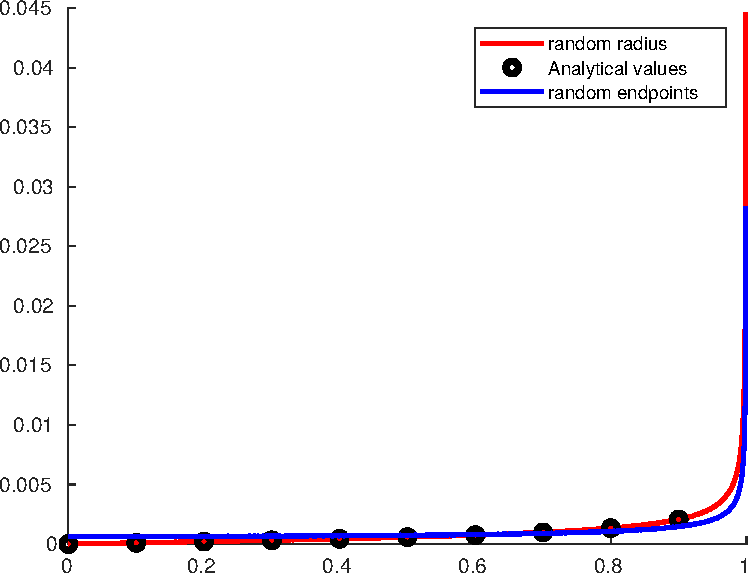
\includegraphics[width=10cm]{disk.pdf}
\caption{Probability of disks chord length simulations in 2-D, equivalent to the radii distribution of the disk, intersections of the sphere and a random plane in 3-D.}
\label{fig:stereology:matlab:disk}
\end{figure}

\subsection{Random planes intersecting a sphere}
\subsubsection{Random radius}
This method is equivalent to the first case of the disk chord. The 3D property of the sphere is not used and thus the code is strictly equivalent to the 2D case.

\begin{matlab}
N = 1e6; % number of points
R = 1; % radius of the sphere
nBins = 1000;

radii = 0:R/nBins:R*(1-1/nBins);

% first simulation: equivalent to a disk
x = R*rand(N, 1);
r = sqrt(R^2 - x.^2);
proba = histcounts(r(r<=R), nBins, 'normalization', 'probability');
\end{matlab}


\subsubsection{Definition of a random intersecting plane by 3 endpoints}
Let $n_1$, $n_2$ and $n_3$ be 3 points on the sphere. These points define the plane $\mathcal{P}$.
The distance between the center of the sphere $O$ and the plane $\mathcal{P}$ is given by the relation:
$$d(0, \mathcal{P})=\frac{|\vec{n}\cdot\vec{u}|}{||\vec{n}||}$$
with $\vec{u}=\vec{n_2}-\vec{n_1}$, $\vec{v}=\vec{n_3}-\vec{n_1}$, and $\vec{n}=\vec{u} \wedge\vec{v}$ the normal vector to the plane. The results are presented in Fig. \ref{fig:stereology:matlab:sphere}.

This is a case of Bertrand's paradox: the definition of randomness is not good in the present case.

\begin{matlab}
% n1, n2 and n3 are 3 arrays of points
n1 = randn(N,3);
mynorm = sqrt(sum(n1.^2,2));
n1 = R* n1 ./ repmat(mynorm,1,3);

n2 = randn(N,3);
mynorm = sqrt(sum(n2.^2,2));
n2 = R* n2 ./ repmat(mynorm,1,3);

n3 = randn(N,3);
mynorm = sqrt(sum(n3.^2,2));
n3 = R* n3 ./ repmat(mynorm,1,3);

% u and v are vectors that belong to the plane
u=n2-n1;
v=n3-n1;
% n: normal vector to the plane
n=cross(u,v);

% x: distance from the center of the sphere to the plane
x = dot(n, n1, 2) ./ sqrt(sum(n.^2, 2));

% r: radius of the intersection sphere/plane
r = sqrt(R^2 - x.^2);

proba = histcounts(r, nBins, 'normalization', 'probability');
plot(radii, proba, 'b');
\end{matlab}


\subsubsection{Use of 2 random points}
This situation presents the random choice of two points on the sphere, and the computation of their distance. This produces a linear probability (see Fig.\ref{fig:stereology:matlab:sphere}).

\begin{matlab}
% first points
n1 = randn(N,3);
mynorm = sqrt(sum(n1.^2,2));
n1 = R* n1 ./ repmat(mynorm,1,3);

% second points
n2 = randn(N,3);
mynorm = sqrt(sum(n2.^2,2));
n2 = R* n2 ./ repmat(mynorm,1,3);

% evaluate half Euclidean distance
r = sqrt(sum((n1-n2).^2, 2))/2;

% probability
proba = histcounts(r, nBins, 'normalization', 'probability');
\end{matlab}


\begin{figure}
 \centering
 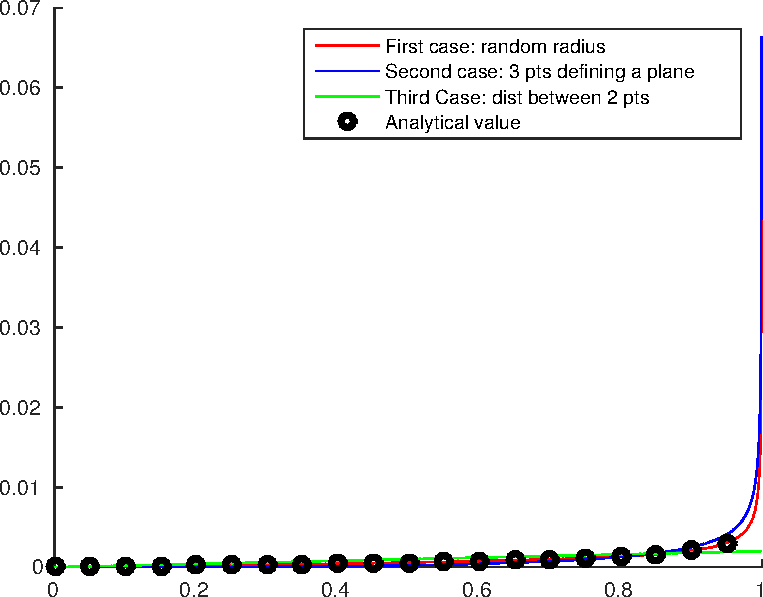
\includegraphics[width=10cm]{sphere.pdf}
 \caption{Case of the sphere intersecting a random plane.}
 \label{fig:stereology:matlab:sphere}
\end{figure}


\begin{note}The Bertrand's paradox is illustrated by the fact that ``at random'' can provide several different interpretations. 
The objective here is to focus on the computational choices that can be made in order to provide random chords or random points on a sphere.\end{note}
